\documentclass[a4paper, 12pt]{article}%тип документа

%отступы
\usepackage[left=2cm,right=2cm,top=2cm,bottom=3cm,bindingoffset=0cm]{geometry}

%Русский язык
\usepackage[T2A]{fontenc} %кодировка
\usepackage[utf8]{inputenc} %кодировка исходного кода
\usepackage[english,russian]{babel} %локализация и переносы

%Вставка картинок
\usepackage{wrapfig}
\usepackage{graphicx}
\graphicspath{{pictures/}}
\DeclareGraphicsExtensions{.pdf,.png,.jpg}

%оглавление
\usepackage{titlesec}
\titlespacing{\chapter}{0pt}{-30pt}{12pt}
\titlespacing{\section}{\parindent}{5mm}{5mm}
\titlespacing{\subsection}{\parindent}{5mm}{5mm}
\usepackage{setspace}

%Графики
\usepackage{multirow}
\usepackage{pgfplots}
\pgfplotsset{compat=1.9}

%Математика
\usepackage{amsmath, amsfonts, amssymb, amsthm, mathtools}

%Заголовок
\usepackage{lastpage} 
\usepackage{fancybox,fancyhdr}
\fancyhead[R]{\textit{Магнитные моменты легких ядер}}
\fancyhead[L]{\textit{Работа 10.4}}
\fancyhead[C]{}

\newtheorem{task}{Задача}
\begin{document}
		\begin{titlepage}
			\begin{center}
				\textit{Федеральное государственное автономное образовательное\\ учреждение высшего образования }
				\vspace{0.5ex}
				
				\textbf{«Московский физико-технический институт\\ (национальный исследовательский университет)»}
			\end{center}
			\vspace{10ex}
			\begin{center}
				\vspace{13ex}
				\textbf{Лабораторная работа №10.4}
				\vspace{1ex}
				
				по курсу основы современной физики
				
				
				на тему:
				
				\textbf{\large{<<Магнитные моменты легких ядер>>}}
				
				\vspace{30ex}
				\begin{flushright}
					\noindent
					\textit{Работу выполнил:}
					\\
					\textit{Валеев Рауф
					}						 
				\end{flushright}
				\vfill
				Долгопрудный \\2021 год
			\end{center}
		\end{titlepage}
	
				\newpage	

	\pagestyle{fancy}

\textbf{Цель работы:} В работе вычисляются магнитные моменты протона, дейтрона и ядра фтора на основе измерения их g-факторов методом ядерного магнитного резонанса (ЯМР). Полученные данные сравниваются с вычислениями магнитных моментов на основе кварковой модели адронов и одночастичной оболочечной модели ядер.

\section{Теоретическое введение}

\subsection{Спин и магнитный момент ядра}
Полный момент количества движения ядра $I$ 	складывается из собственной (спиновой) $S$ и орбитальной $L$ частей.
\[I = L + S\]
Согласно квантовой механике, полный момент количества движения $I$ изолированной системы (ядра) принимает (в единицах $\hbar$) целые или полуцелые значения.

Отношение магнитного момента ядра $\mu_{\text{я}}$ к механическому моменту $I$ задается гиромагнитным отношение
\[\mu=g_{\text{я}}\mu_{\text{я}}I\]
Где $g_{\text{я}}$– ядерный $g$-фактор, $\mu_{\text{я}}$– ядерный магнетон, I измеряется в величинах $\hbar$.
\[\mu_{\text{я}} = \frac{e\hbar}{2 M c}\]
M – масса протона. 

Таким образом, для вычисления магнитного момента ядра необходимо определить величину его механического момента и $g$-фактора. В данной работе для определения величины $g$-фактора используется метод ядерного магнитного резонанса (ЯМР).

\subsection{Сверхтонкая структура оптических спектров}
Сверхтонкая структура спектров вызвана взаимодействием электронов с магнитным моментом ядра. В результате взаимодействия магнитного момента ядра с магнитным полем, создаваемым движением электронов в атомной оболочке, электроны приобретают дополнительную энергию, зависящую от величины магнитного момента ядра и его ориентации относительно направления магнитного поля электрона. Величина $I$ определяется путем простого подсчета числа компонент сверхтонкой структуры в спектре данного изотопа.
\subsection{Чередование интенсивностей в полосатых спектрах двухатомных молекул с тождественными ядрами}
Этот метод дает возможность определить I. Чередование интенсивностей является следствием того, что волновая функция молекулы с тождественными ядрами должна быть либо симметричной либо антисимметричной относительно перестановки координат и спина. Определение I основано на том факте, что статистические веса симметричных и антисимметричных состояний относятся как $(I+1)/I$.
\subsection{Ядерные реакции}
Если известен спин начального ядра, а затем происходит некоторый распад, то можно сделать определенные выводы относительно спина конечного ядра, и наоборот. Основано такое определение спина на том, что вероятность перехода(т.е. время жизни возбужденного состояния) зависит от спина и четности исходного и конечного ядра. Разность спинов и четностей этих состояний может быть определена по измерению углового распределения вылетающих $\gamma$-квантов.
\subsection{Ядерный магнитный резонанс}
ЯМР – это резонансное поглощение электромагнитной энергии в веществах, обусловленное ядерным перемагничиванием. ЯМР наблюдается в постоянном магнитном поле $B_0$ при одновременном воздействии на образец радиочастотного магнитного поля, перпендикулярного $B_0$ и обнаруживается по поглощению излучения. У нейтральных атомов в сильном магнитном поле связь между $I$ и $J$ разрывается, и оба эти вектора независимо прецессируют с одинаковой угловой частотой $w=g\frac{eH}{Mc}$, где $g$- гиромагнитное отношение. Если теперь наложить слабое добавочное поле $H’$, перпендикулярное к основному полю, то оно вызовет изменение ориентации ядреных спинов.

\section{Экспериментальная установка}
\begin{figure}[h]
\begin{center}
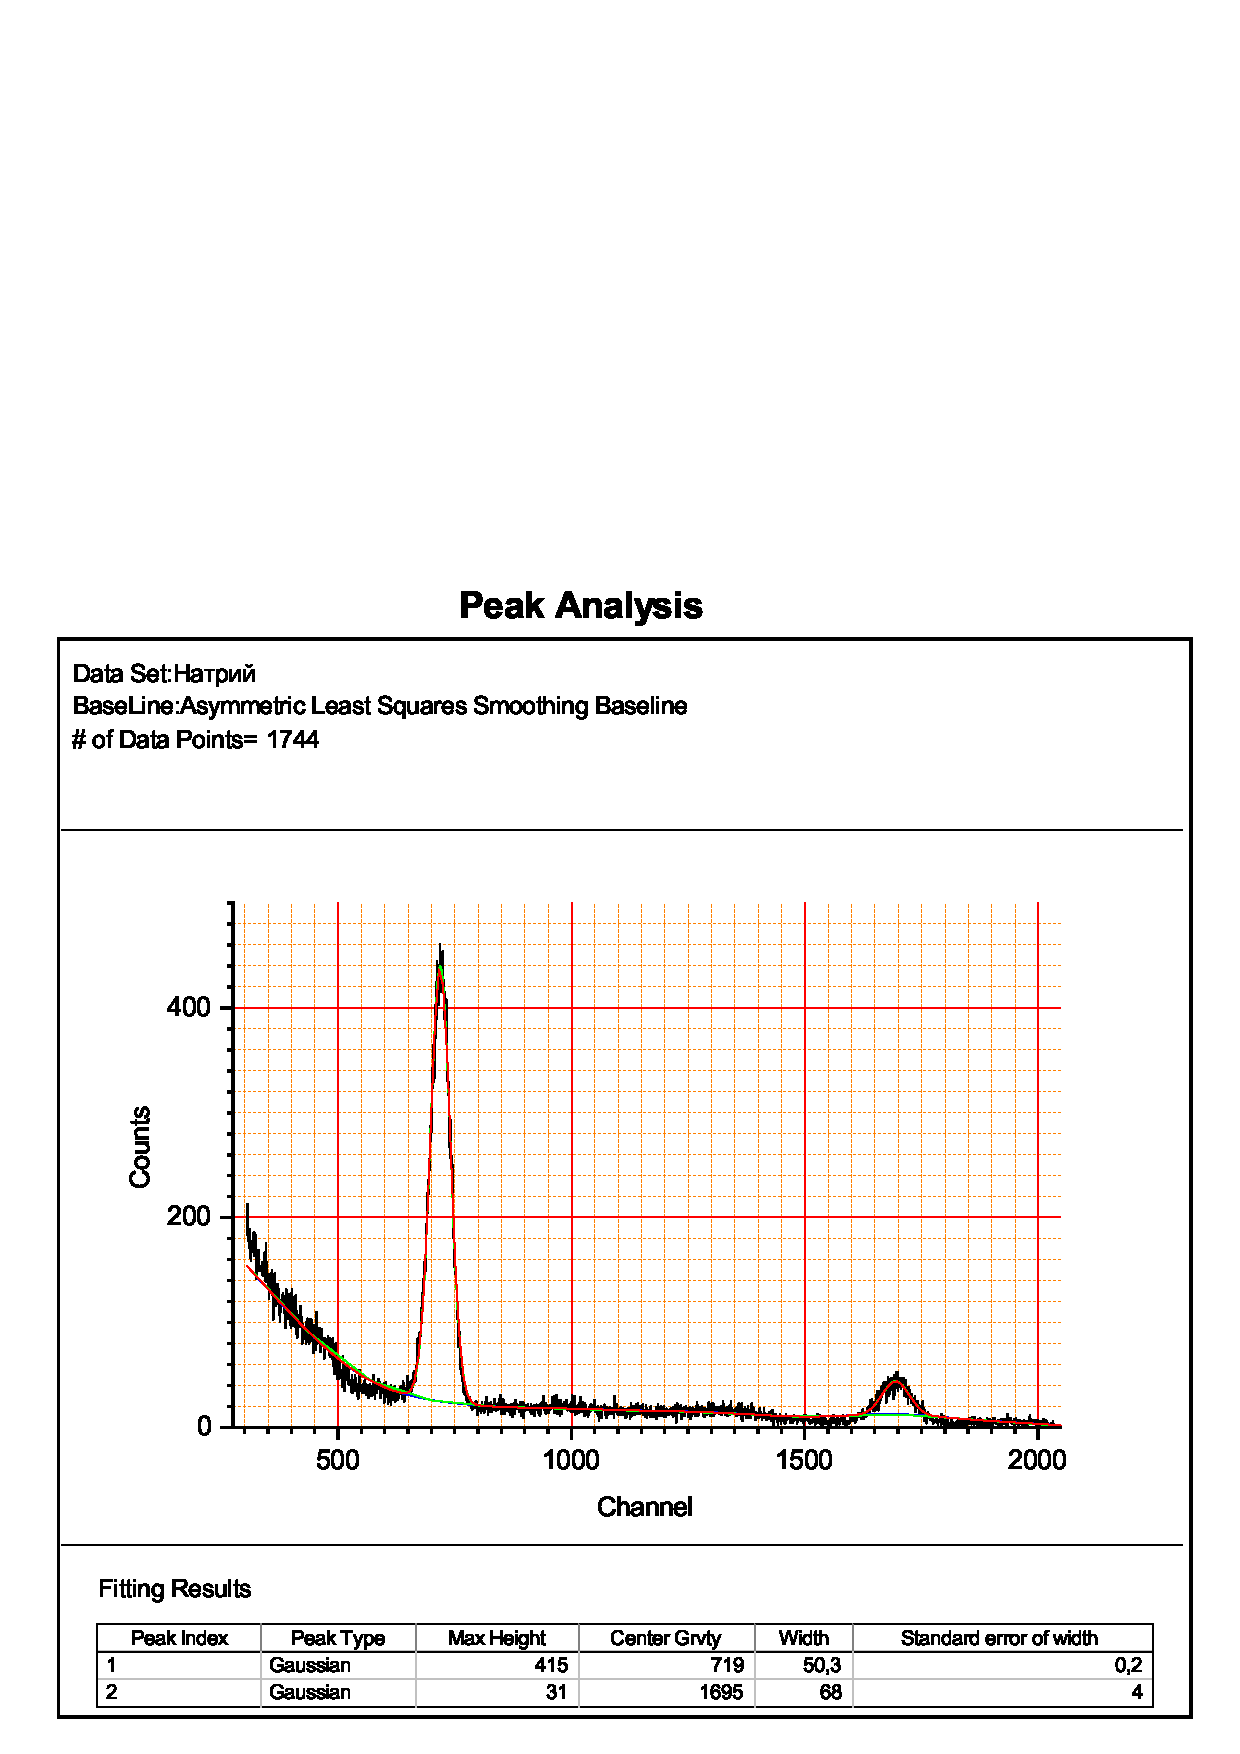
\includegraphics[width = \textwidth]{1.jpg}
\caption{Схема установки для изучения ядерного магнитного резонанса}
\end{center}
\end{figure}
В магнитном поле ядерные уровни расщепляются и под действием внешнего высокочастотного поля могут происходить электромагнитные переходы между компонентами расщепившегося уровня, это явление носит резонансный характер и потому называется ядерным магнитным резонансом. Различие по энергии между этими двумя соседними компонентами определяется формулой
\[\Delta E = g_{\text{я}}\mu_{\text{я}}B_0\]
\[f_0 = \frac{\Delta E }{h} = \frac{g_{\text{я}}\mu_{\text{я}}B_0}{h}\]

Схема экспериментальной установки представлена на рис. 1. Детектирование сигнала ЯМР осуществляется с помощью промышленного прибора. Модуляция магнитного поля осуществляется с помощью небольшой катушки, частота модуляции $\approx 50$ Гц. В зазоре электромагнита устанавливается холловский измеритель магнитного поля, а измерения ЯМР проводятся на резине (измеряется ЯМР на протонах), тефлоне (в состав входит фтор) и тяжелой воде.
\section{Измерения. Анализ результатов}
\begin{table}[h]
\begin{center}
\begin{tabular}{|c|c|c|c|}
\hline
                      & Вода   & Резина & Тефлон \\ \hline
$f_0$, МГц            & 9,86   & 9,90   & 9,72   \\ \hline
$\sigma_{f_0}$, МГц   & 0,01   & 0,01   & 0,01   \\ \hline
$B_0$, мТл            & 231,62 & 232,55 & 229,62 \\ \hline
$\sigma_{B_0}$, мТл   & 0,01   & 0,01   & 0,01   \\ \hline
$I$, A                & 0,32   & 0,35   & 0,36   \\ \hline
$V$, В                & 18,6   & 20,2   & 20,6   \\ \hline
$B_0$ холла, мТл    & 231    & 232    & 243    \\ \hline
$\sigma_{B_0}$, мТл   & 1      & 1      & 1      \\ \hline
$g$                   & 5,6    & 5,6    & 5,25   \\ \hline
$\sigma_g$            & 0,02   & 0,02   & 0,02   \\ \hline
$\mu$, $\mu_{\text{я}}$        & 2,80   & 2,80   & 2,625  \\ \hline
$\sigma_{\mu}$, Дж/Тл & 0,01   & 0,01   & 0,01   \\ \hline
\end{tabular}
\caption{Измеренные величины и итоговые $g$-факторы и угловые моменты для разных веществ}
\end{center}
\end{table}

\begin{figure}[h]
\begin{center}
\includegraphics[width = 0.4\textwidth]{21.jpg}
\includegraphics[width = 0.4\textwidth]{22.jpg}
\caption{Тефлон и Вода}
\end{center}
\end{figure}

\begin{figure}[h]
\begin{center}
\includegraphics[width = 0.4\textwidth]{23.jpg}
\caption{Резина}
\end{center}
\end{figure}
В образцах тефлон и вода исследуется ЯМР на протонах, поскольку формула для ядерного $g$-фактора уже приведена в теории, как и формула для вычисления величины углового момента, то нам не хватает, для их вычисления, только спинового числа. Поскольку ЯМР на протонах, то спиновое число равно 1/2, и из этого мы легко считаем все, что нам надо.

Аналогично вычисляется величина $g$-фактора ядра фтора, а затем его магнитный момент. Величина $g$-фактора и магнитного момента близка к значению для протона, так как орбитальное движение протона не вносит вклад в магнитный момент этого ядра, и он определяется только спином протона.

В итоге, зная что табличные значения для протона и фтора соответственно равны:
\[\mu_P = 2,7928 \mu_{\text{я}}\]
\[\mu_F = 2,6258 \mu_{\text{я}}\]

То мы видим, что у нас идеально совпадает эксперимент с теорией.
\section{Вывод}
В ходе работы были вычислены магнитные моменты протона, дейтрона и ядра фтора на основе измерения их $g$-факторов методом ядерного магнитного резонанса (ЯМР). Полученные данные сравнивались с вычислениями магнитных моментов на основе кварковой модели адронов и одночастичной оболочечной модели ядер.

В результате:
\begin{enumerate}
\item 
Магнитный момент и $g$-фактор протона хорошо согласуются с табличными значениями;
\item
Значения магнитного момента и $g$-фактора ядра фтора оказались близки к соответствующим значениям для протона, как и предсказывает теория.


\end{enumerate}
\end{document}
